\subsection{ARIMA, SARIMA e SARIMAX}\label{subsec:arima}

A previsão da série temporal é um problema difícil sem resposta fácil. Existem inúmeros modelos estatísticos que afirmam superar uns aos outros, mas nunca está claro qual modelo é o melhor.

Dito isto, modelos baseados em ARMA são muitas vezes um bom modelo para começar. Eles podem alcançar pontuações decentes na maioria dos problemas de séries temporais e são bem adequados como um modelo de linha de base em qualquer problema de séries temporais.


O modelo ARIMA, vamos dividi-lo em AR, I e MA.

\subsubsection{Componente Autorregressivo}

O componente auto regressivo do modelo ARIMA é representado por AR(p), com o parâmetro $ p $ determinando o número de séries defasadas que é utilizado.

\begin{eqnarray}
	Y_t&=&c+\sum_{n=1}^{p} \alpha_n y_{t-n} + \varepsilon_t\label{AR}
\end{eqnarray}

Dos dados pode ser obtido a seguinte previsão no modelo AR(7)

\begin{figure}[H]
	\centering
	\caption{Modelo AR(7)  }
	\label{fig:1-ar}
	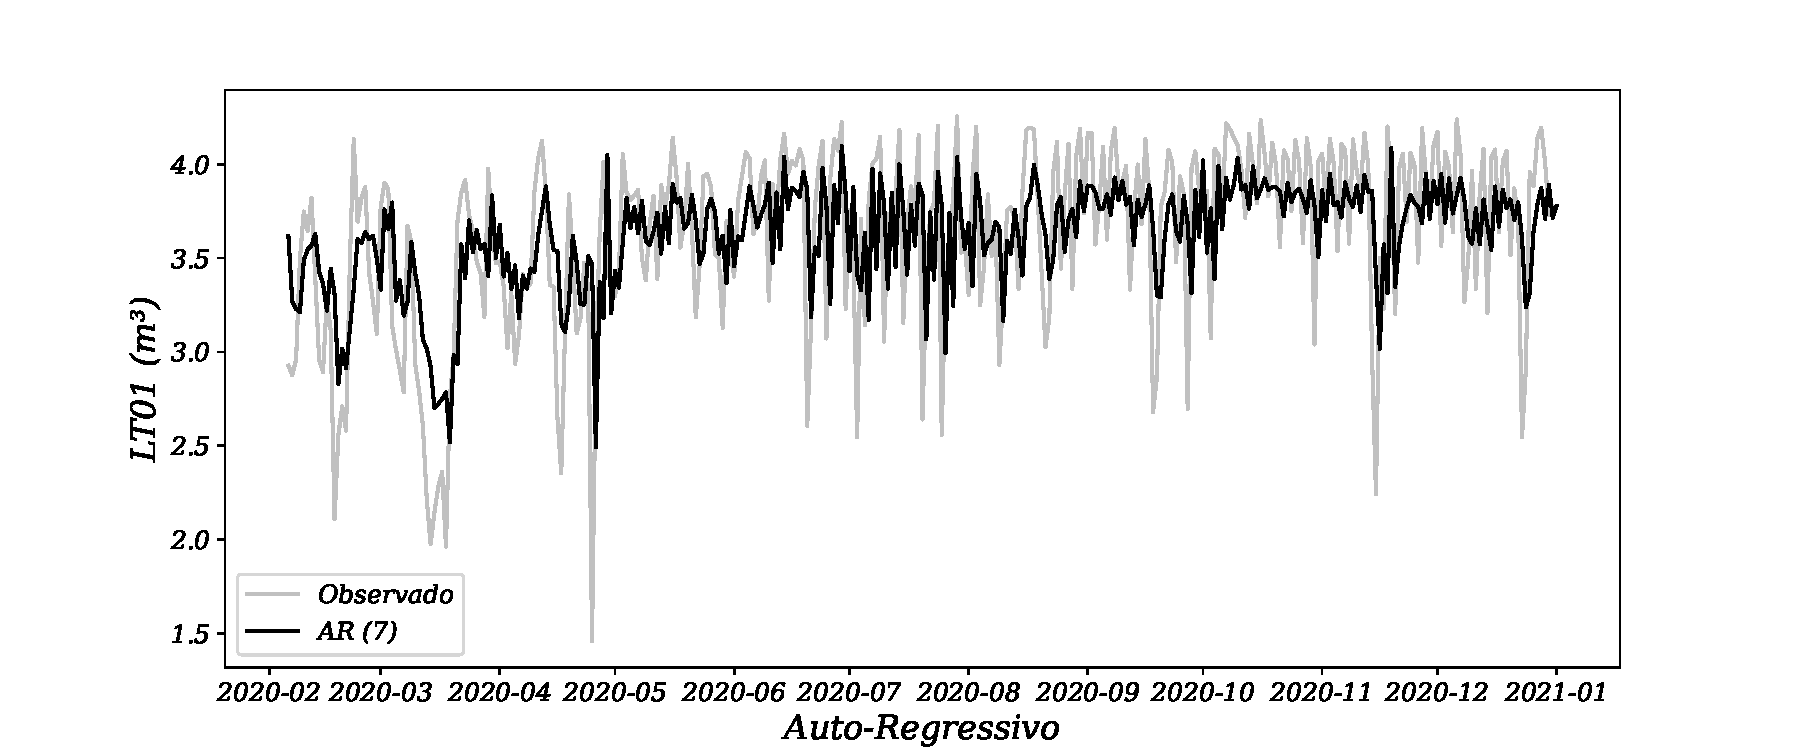
\includegraphics[width=0.9\linewidth]{Modelos/Figuras/0-AR}
	
	Fonte: Elaboração própria a partir de dados da SANEPAR (2018 a 2020)
\end{figure}

\begin{figure}[H]
	\centering
	\caption{ARX (7)}
	\label{fig:1-arx}
	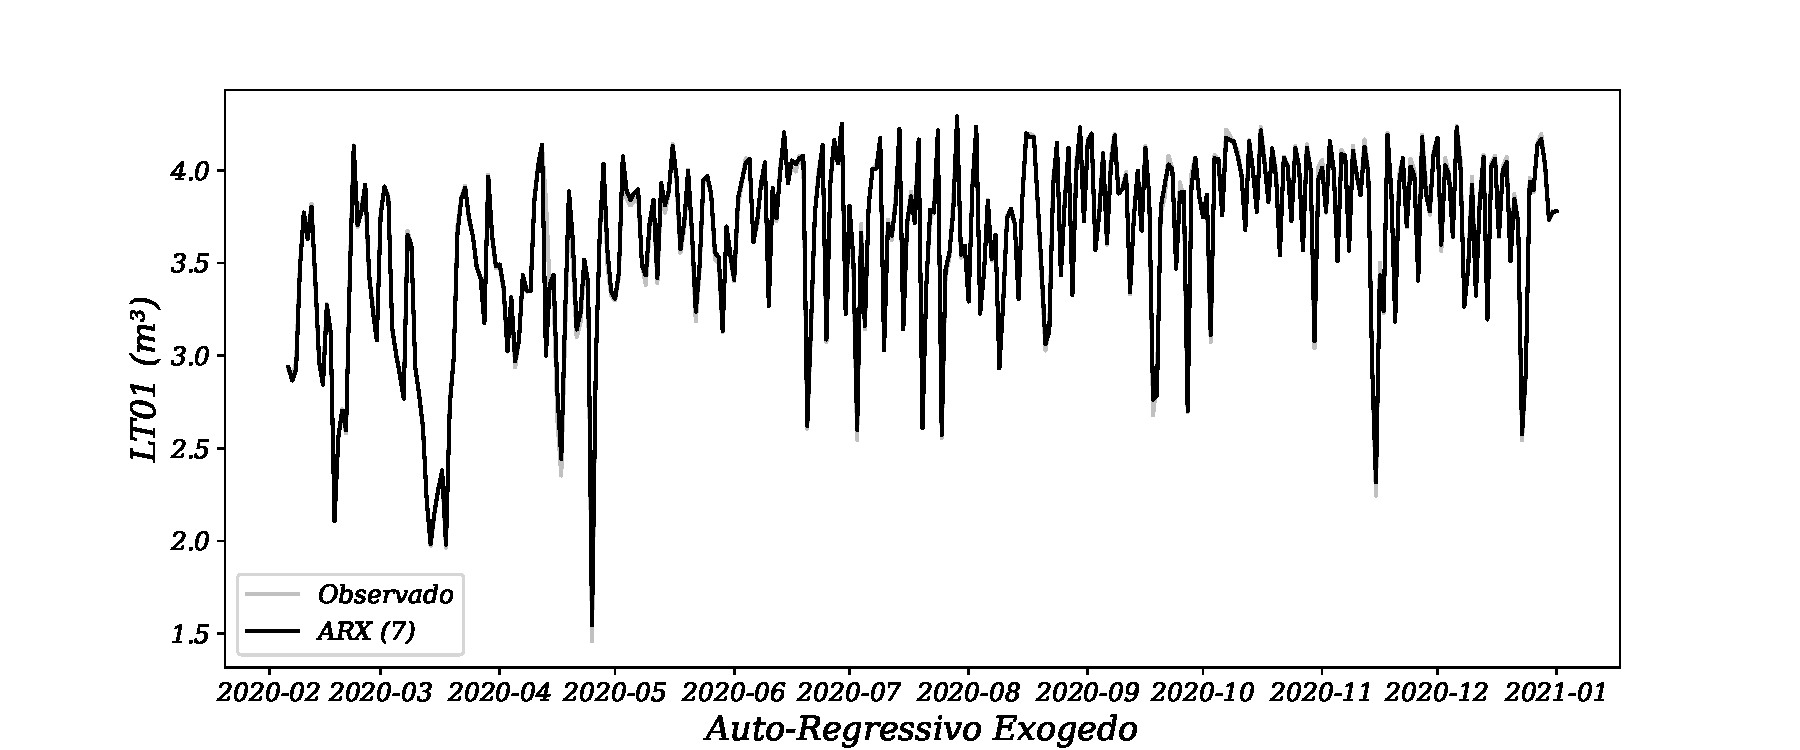
\includegraphics[width=0.9\linewidth]{Modelos/Figuras/0-ARX}
	
	Fonte: Elaboração própria a partir de dados da SANEPAR (2018 a 2020)
\end{figure}



Onde em \eqref{AR} o $\varepsilon_t$ é ruído branco. Isso é como uma regressão múltipla, mas com valores defasados de $y_t$ como preditores. é referido a isso como um $\operatorname{AR}(p)$ modelo, um modelo auto regressivo de ordem $p$

Da Figura \ref{fig:1-ar}, tem como objetivo mostrar uma previsão de um passo a frente (um dia) nos apêndices \ref{sec:ararxma24} pode ver uma comparação dos AR, MA e o ARX

O modelo ARX é um modelo similar ao AR só coloca as variáveis exógenas do conjunto de dados para melhorar a previsão futura.

O modelo AR pode ser visivelmente um modelo adequado para a previsão que está sendo feito, mas como é um modelo auto regressivo ainda assim com o passar do tempo e da previsão ele vai prever de uma forma linear e não convencional, para um analise mais rápido da série pode se considerar um modelo adequado. Logo mais adiante tem exemplos de casos gerais que pode ocorrer nesse método.

\subsubsection{AR(0): Ru\'ido branco}

Se definir o parâmetro $p$ como zero (AR($0$)), sem termos autorregressivos. Esta série de tempo é apenas um ruído branco. Cada ponto de dados é amostrado a partir de uma distribuição com uma média de $0$ e uma variância de sigma-quadrado. Isso resulta em uma sequência de números aleatórios que não podem ser previstos. Isso é realmente útil, pois pode servir como uma hipótese nula, e proteger nossas análises de aceitar padrões falso-positivos.

\subsubsection{AR(1): Caminhadas aleat\'orias e Oscila\c c\~oes}



Com o parâmetro p definido para $1$, vai levar em conta o medidor de tempo anterior ajustado por um multiplicador e, em seguida, adicionando ruído branco. Se o multiplicador é $0$, então temos ruído branco, e se o multiplicador é 1, teremos uma caminhada aleatória. Se o multiplicador estiver entre $ 0 < \alpha < 1 $, então a série temporal exibirá reversão média. Isso significa que os valores tendem a pairar em torno de 0 e reverter para a média depois de regredir a partir dele.

\subsubsection{AR(p): Termos de ordem superior}

Aumentar ainda mais o parâmetro $p$ significa apenas ir mais para trás e adicionar mais medidores de tempo ajustados por seus próprios multiplicadores. Pode ir o mais longe que poder, mas à medida que aproxima é mais provável que usa parâmetros adicionais, como a média móvel (MA($q$)).

\subsubsection{M\'edia M\'ovel}\label{subsubsec:ma}
Este componente não é uma média de rolamento, mas sim os atrasos no ruído branco. \citeonline{signal}


MA(q) é o modelo de média móvel e q é o número de termos de erro de previsão defasados na previsão. Em um modelo MA(1), na previsão é um termo constante mais o termo de ruído branco anterior vezes um multiplicador, adicionado com o termo de ruído branco atual. Esta é apenas simples probabilidade mais estatísticas, pois estamos ajustando nossa previsão com base em termos anteriores de ruído branco.

\begin{eqnarray}
	y_t=c+\varepsilon_t+\theta_1 \varepsilon_{t-1}+\theta_2 \varepsilon_{t-2}+\cdots+\theta_q \varepsilon_{t-q}\label{eq:ma}
\end{eqnarray}

De \eqref{eq:ma} onde $\varepsilon_t$ é ruído branco. Refere nos a isto como um modelo de $MA(q)$, um modelo de ordem média móvel $q$. Claro que não observamos os valores de $\varepsilon_t$, por isso não é realmente uma regressão no sentido habitual.

\begin{figure}[H]
	\centering
	\caption{Modelo MA(7) }
	\label{fig:1-ma}
	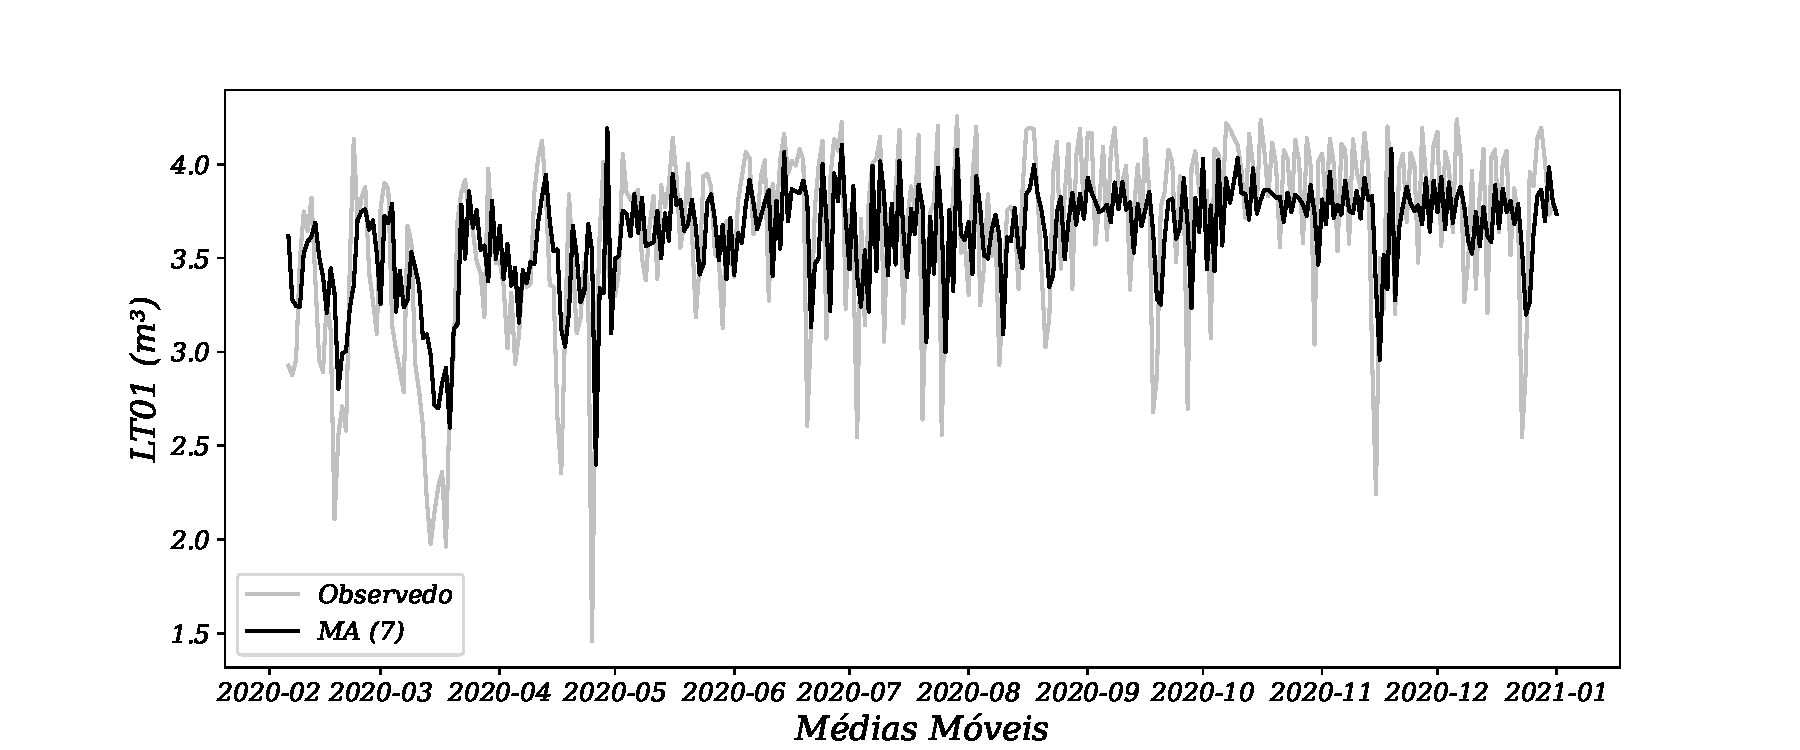
\includegraphics[width=0.9\linewidth]{Modelos/Figuras/0-MA}
	
	Fonte: Elaboração própria a partir de dados da SANEPAR (2018 a 2020)
\end{figure}

O modelo MA com o mesmo valor do AR para comparação e torna o modelo mais fácil de ser previsto. Como observado na Figura \ref{fig:1-ma} a previsão graficamente é parecido com o modelo da Figura \ref{fig:1-ar}, só não se compara com a Figura \ref{fig:1-arx}, perceba que esse modelo aparente prever perfeitamente o tempo que foi listado.  

\subsubsection{Modelos ARMA e ARIMA}\label{subsubsec:arma}
As arquiteturas ARMA e ARIMA são apenas os componentes AR (Autoregressive) e MA (Moving Average) juntos.

\subsubsection{ARMA}

O modelo ARMA é uma constante mais a soma de lags AR e seus multiplicadores, além da soma dos lags ma e seus multiplicadores mais ruído branco. Esta equação é a base de todos os modelos que vêm a seguir e é uma estrutura para muitos modelos de previsão em diferentes domínios.

\begin{figure}[H]
	\centering
	\caption{ARMA (7,7)}
	\label{fig:1-arma}
	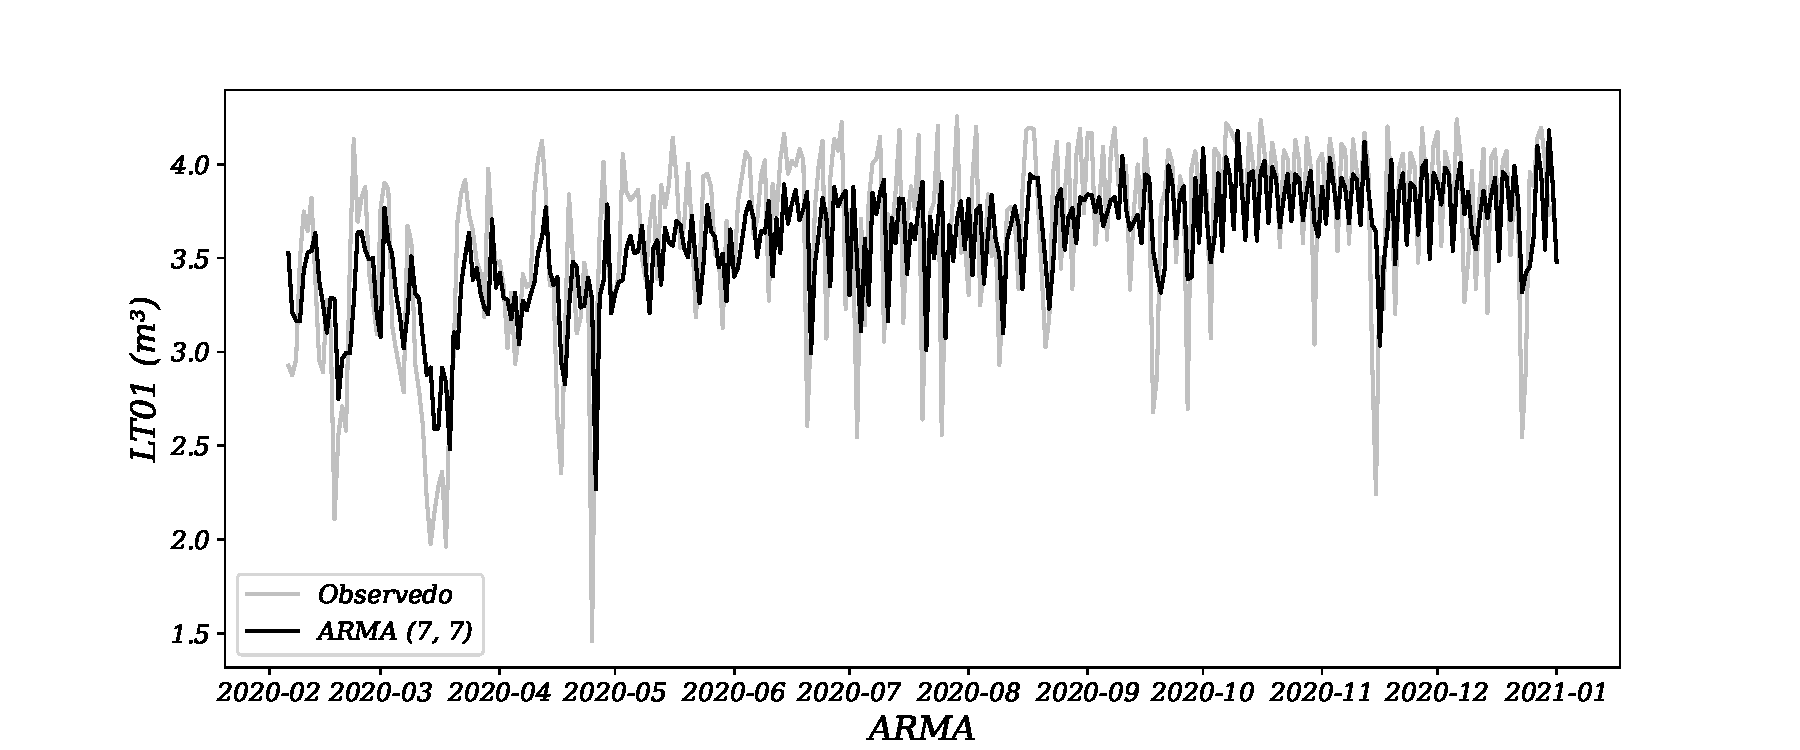
\includegraphics[width=0.9\linewidth]{Modelos/Figuras/0-ARMA}
	
	Fonte: Elaboração própria a partir de dados da SANEPAR (2018 a 2020)
\end{figure}

Da Figura \ref{fig:1-arma} é a junção dos modelos AR e MA esse modelos juntos pode ocorrer a redução do erro em escala mais significativa, nos apêndice \ref{sec:comtb24} e \ref{sec:comtb18} pode ser notado a comparação de alguns passos a mais do que mostrado aqui.

\subsubsection{ARIMA}

\begin{eqnarray}
	Y_t = \beta_2 + \omega_1\varepsilon_{t-1} + \omega_2 \varepsilon_{t-2} +\ldots+ \omega_q \varepsilon_{t-q} + \varepsilon_t \label{arima}
\end{eqnarray}


Onde em \eqref{arima} o $Y_t$ é a série diferenciada (pode ter sido diferente mais de uma vez). Os ``preditores" no lado direito incluem ambos os valores defasados de $Y_t e$ erros defasados. Chamamos isso de ARIMA( $p, d, q$ ).

O modelo ARIMA é um modelo ARMA ainda com uma etapa de pré-processamento incluída no modelo que representamos usando I(d). I(d) é a ordem de diferença, que é o número de transformações necessárias para tornar os dados estacionários. Assim, um modelo ARIMA é simplesmente um modelo ARMA na série de tempo diferente.

\begin{figure}[H]
	\centering
	\caption{ARIMA (7,1,7)}
	\label{fig:1-arima}
	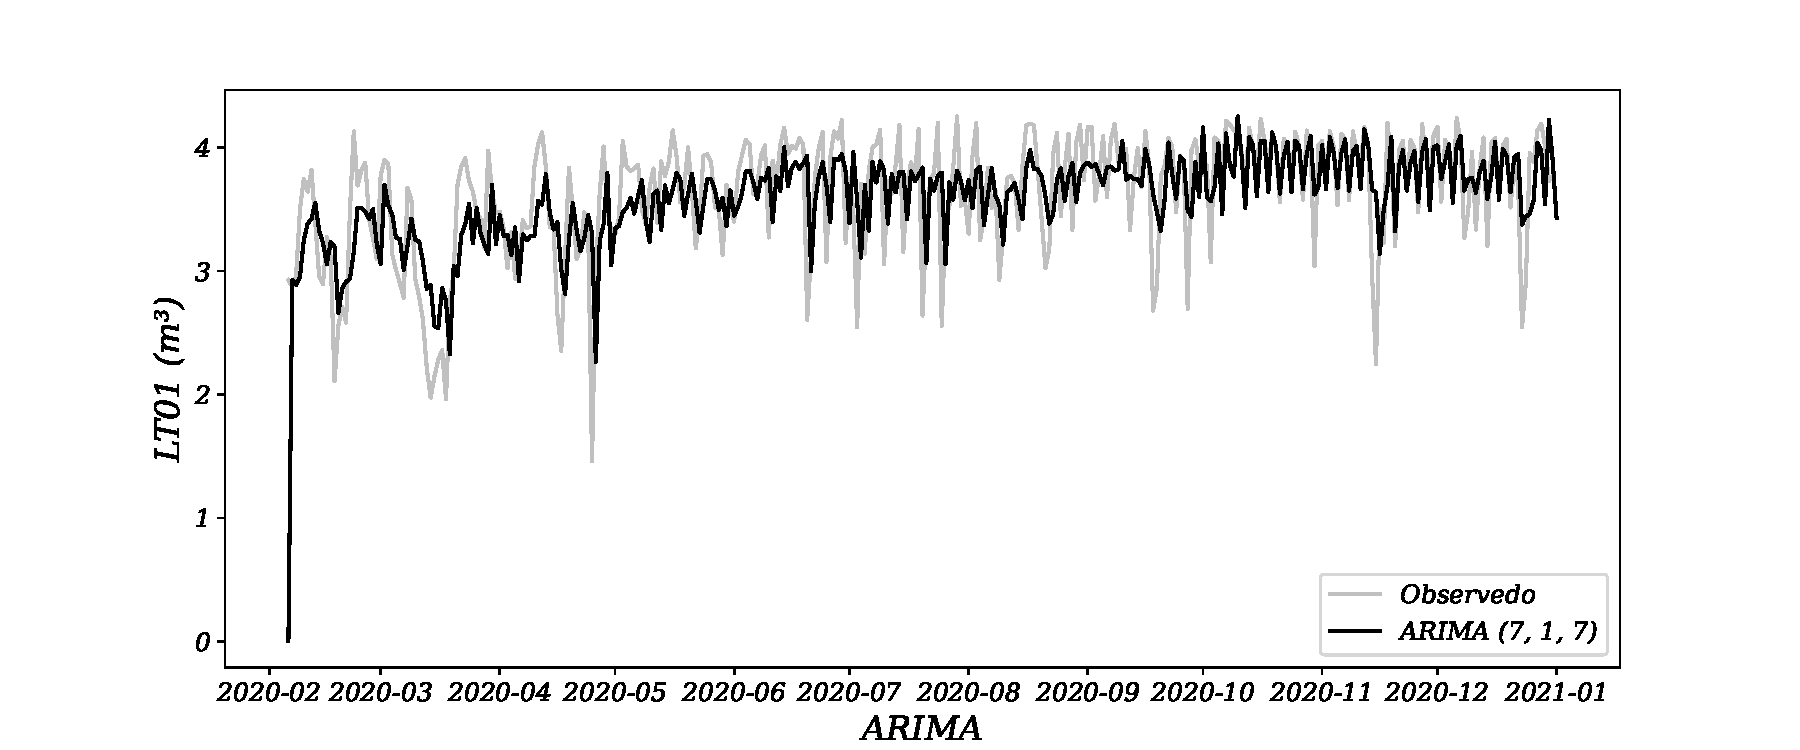
\includegraphics[width=0.9\linewidth]{Modelos/Figuras/0-ARIMA}
	
	Fonte: Elaboração própria a partir de dados da SANEPAR (2018 a 2020)
\end{figure}

Olhando a Figura \ref{fig:1-arima} podemos perceber que não tem muita diferença visual com os outros métodos mostrados até agora, visualmente o método ARX ainda esta melhor que os outros.  


\subsubsection{Modelos SARIMA, ARIMAX e SARIMAX}

Os modelos ARIMA são ótimos, mas incluir variáveis sazonais e exógenas no modelo pode ser muito poderoso. Como o modelo ARIMA assume que a série temporal é estacionária, precisamos usar um modelo diferente.
\textbf{SARIMA}

\begin{eqnarray}
	Y_t&=&c+\sum_{n=1}^p \alpha_n y_{t-n}+\sum_{n=1}^q \theta_n \epsilon_{t-n}+\sum_{n=1}^P \phi_n y_{t-s n}+\sum_{n=1}^Q \eta_n \epsilon_{t-s n}+\epsilon_t \label{sarima}
\end{eqnarray}

O modelo é muito semelhante ao modelo ARIMA, com um conjunto adicional de componentes autorregressivos e de média móvel. O atraso extra é compensado pela frequência sazonal (por exemplo, 12 - mensal, 24 - por hora). 

\begin{figure}[H]
	\centering
	\caption{SARIMA $(7,1,7) (2,1,1)_{12}$}
	\label{fig:1-sarima}
	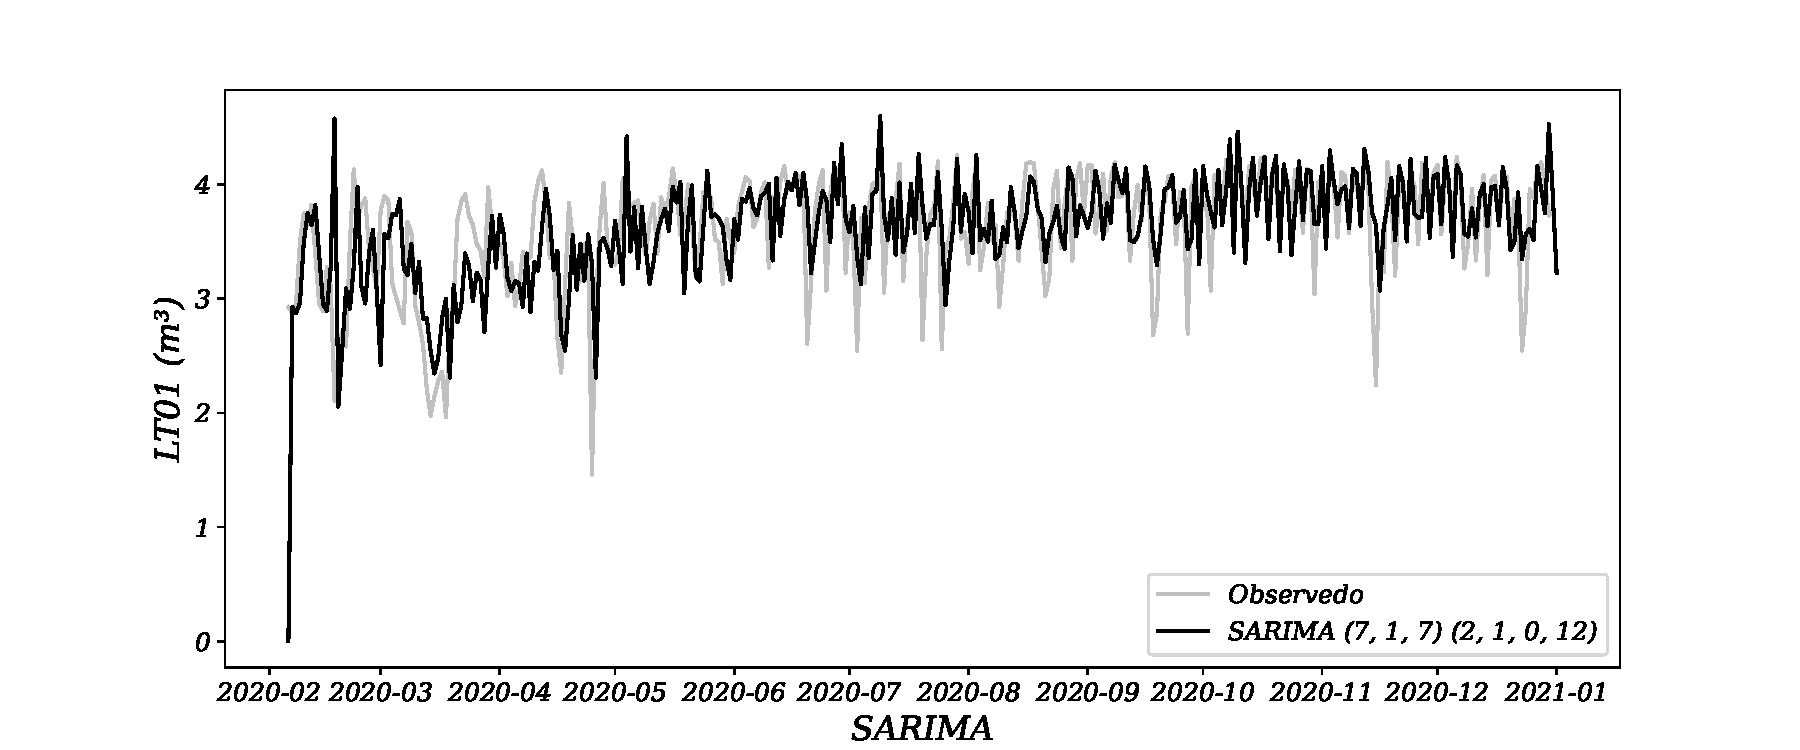
\includegraphics[width=0.9\linewidth]{Modelos/Figuras/0-SARIMA}
	
	Fonte: Elaboração própria a partir de dados da SANEPAR (2018 a 2020)
\end{figure}

Na Figura \ref{fig:1-sarima} pode ser observado como a previsão em vermelho esta mais próxima do observado em preto, só acionando o termo de sazonalidade na previsão. 

Os modelos SARIMA permitem diferenciar dados por frequências sazonais e não sazonais. Uma estrutura de pesquisa automatizada de parâmetros, como pmdarina, pode ajudar a entender quais são os melhores parâmetros.

\textbf{ARIMAX e SARIMAX}

\begin{eqnarray}
	d_t=c+\sum_{n=1}^p \alpha_n d_{t-n}+\sum_{n=1}^q \theta_n \epsilon_{t-n}+\sum_{n=1}^r \beta_n x_{n_t}+\sum_{n=1}^P \phi_n d_{t-s n}+\sum_{n=1}^Q \eta_n \epsilon_{t-s n}+\epsilon_t \label{eq:sarmax}
\end{eqnarray}

Em \eqref{eq:sarmax} está o modelo SARIMAX. Este modelo tem em conta variáveis exógenas, ou por outras palavras, utiliza dados externos na nossa previsão. É interessante pensar que todos os factores exógenos ainda são tecnicamente indiretamente modelados na previsão histórica do modelo. Dito isto, se incluirmos dados externos, o modelo responderá muito mais rapidamente ao seu efeito do que se confia na influência de termos desfasados.

\begin{figure}[H]
	\centering
	\caption{ARIMAX $(7,1,7)$  }
	\label{fig:1-arimax}
	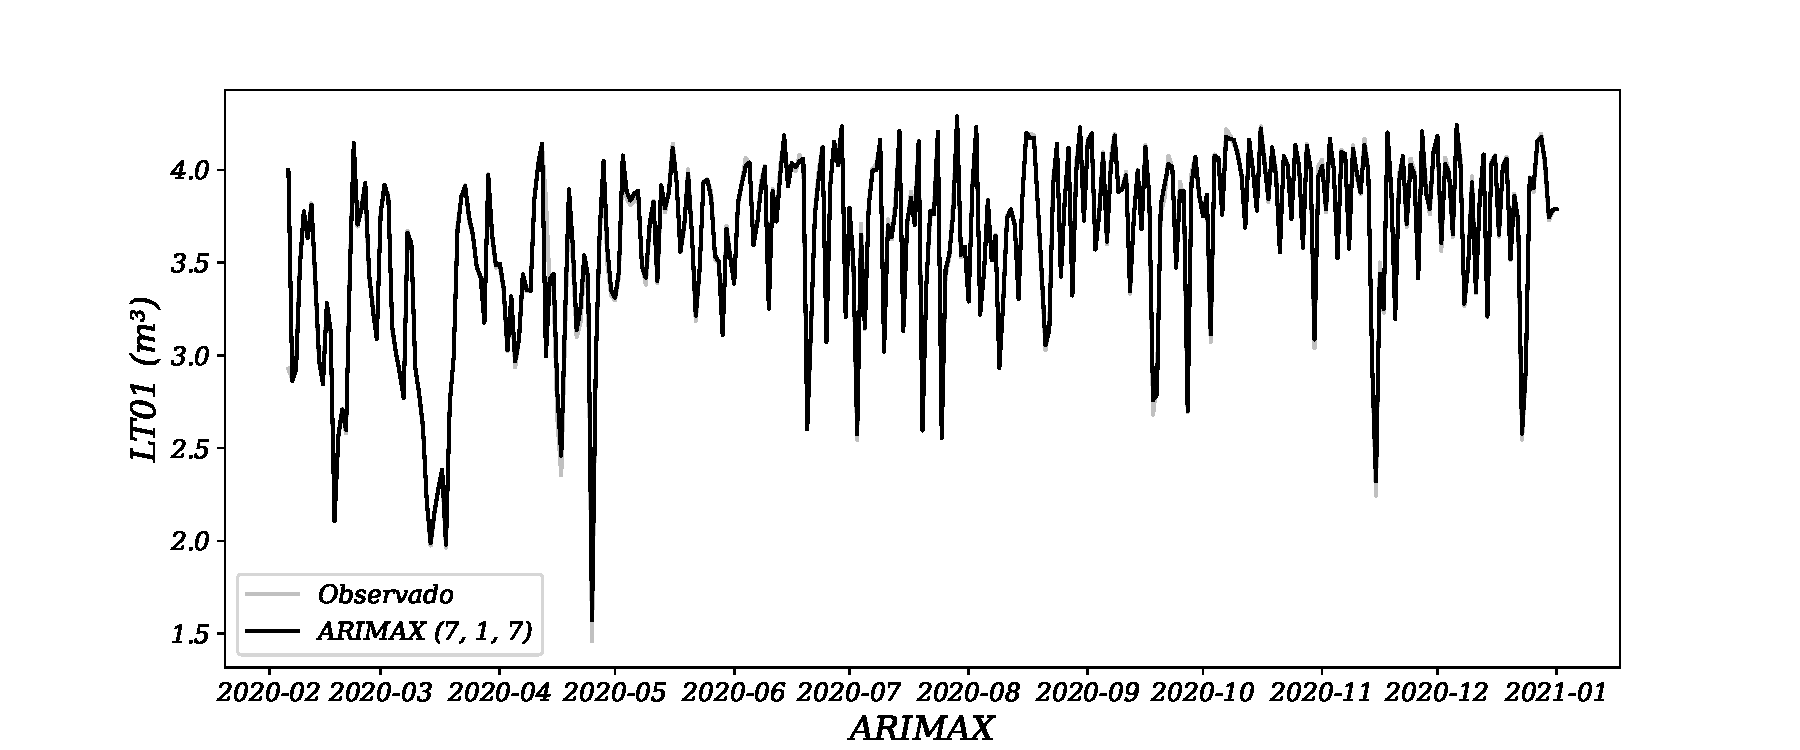
\includegraphics[width=0.9\linewidth]{Modelos/Figuras/0-ARIMAX}
	
	Fonte: Elaboração própria a partir de dados da SANEPAR (2018 a 2020)
\end{figure}

\begin{figure}[H]
	\centering
	\caption{SARIMAX $(7,1,7) (2,1,1)_{12}$  }
	\label{fig:1-sarimax}
	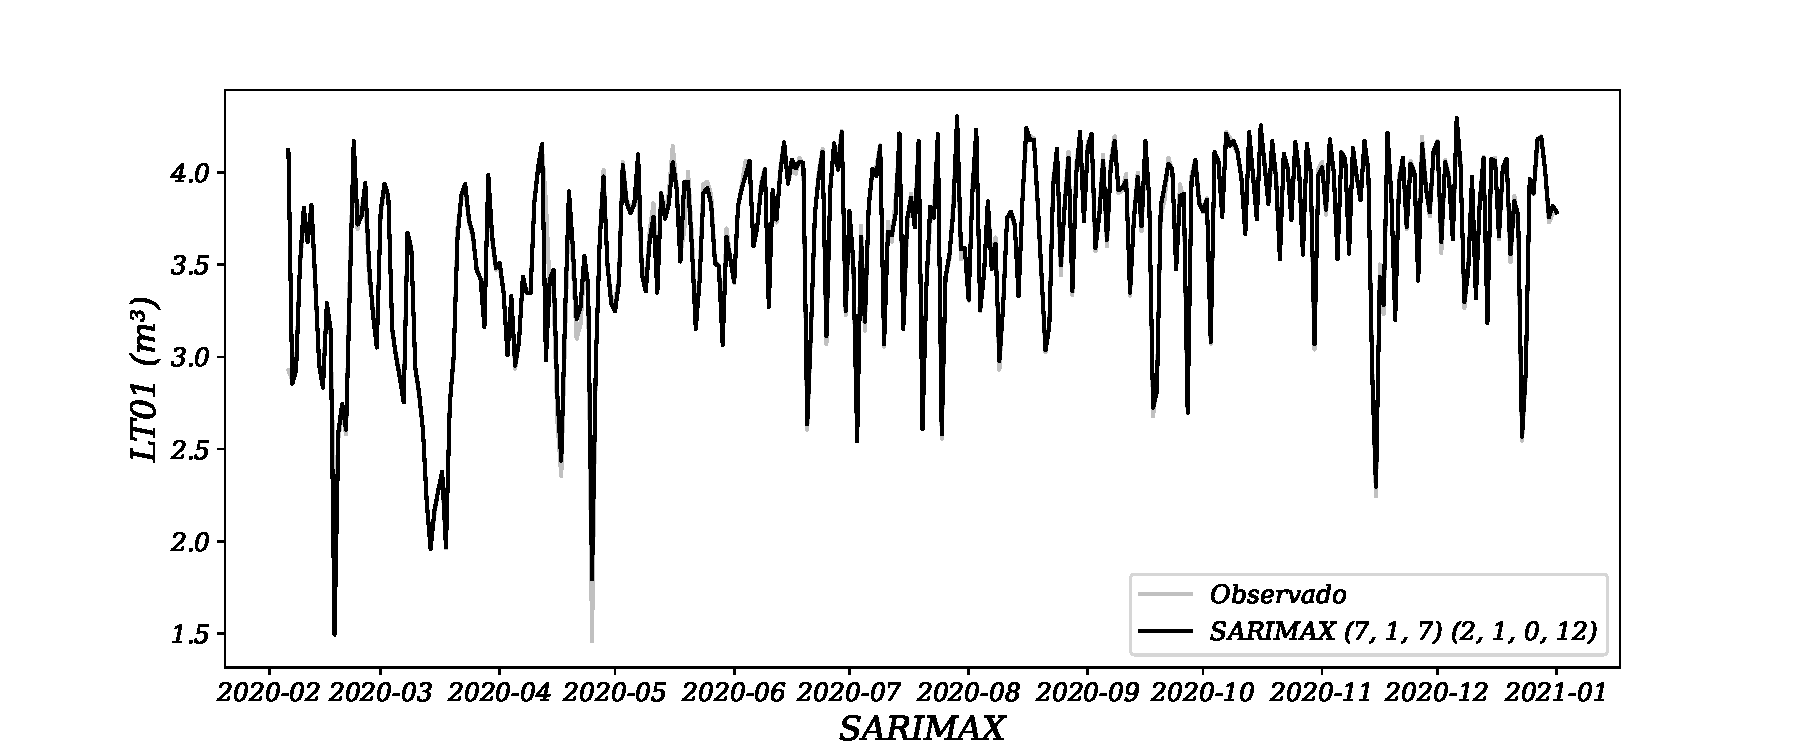
\includegraphics[width=0.9\linewidth]{Modelos/Figuras/0-SARIMAX}
	
	Fonte: Elaboração própria a partir de dados da SANEPAR (2018 a 2020)
\end{figure}


Entre os modelos com variáveis exógenas os modelos da Figura \ref{fig:1-arimax} e \ref{fig:1-sarimax}, é possível perceber que a previsão está mais completa do que nos modelos sem a variável exógena.
